\chapter{Credential Certification Mechanism\label{cha:chapter3}}

\begin{displayquote}
``\textit{What is all knowledge except recorded experience}'' \\- Thomas Carlyle (1795 - 1881)
\end{displayquote}
% observed philosopher 

The Semantic Web has been described as heralding the age of ``Web 3.0''. 
Increasingly this accolade is applied to blockchain technologies.
This chapter focuses on the problem of recognizing achievement in the emerging realm of massive open online courses (MOOCs) in addition to other non-traditional educational environments, to demonstrate the practical applicability of our approach. 
We evaluate the technical work we have undertaken towards realization of the benchmarks described in the previous section with the introduction of a blockchain-based decentralized application for the certification of academic credentials. 
Although blockchain is a relatively recent phenomena it draws on a rich history of pioneering research. Recognizing the achievements of our peers, and the industrial efforts in the domain, we consider the related work and juxtapose it with our own implementation.

% \autoref{fig:passport} depicts a scenario of how a smart contract platform such as Ethereum could support micro and standard accreditation within a higher educational setting. Educational establishments including universities and MOOC companies such as FutureLearn develop and deploy courses and award recognition of student achievement through certificates, micro-certificates and badges. 
% Students take courses and gain recognition after registering for and completing courses through certification. 
% In an era of re-skilling and lifelong learning\footnote{\footnotesize{No 21 year old on completion of a bachelor's degree will have gained all the skills he or she requires for the rest of his/her life}} students will increasingly take a variety of courses from a variety of providers over a longer period of time. There is a need in this context for students to be able to collect and store all their informal and formal qualifications in a fashion that makes these easily accessible to relevant parties such as potential employers and educational organisations. 
% The above process can be supported by two decentralized blockchain based applications (\DJ{}Apps) running on the Ethereum network. A Certificate Issuing and Validation \DJ{}App would handle the publication of signed certificates within a blockchain. Secure signatures would tie all certificates to the specific issuing educational institution and the receiving student. Because of the nature of blockchains the certificates would remain valid even if the issuing organisation ceased to exist. Recently, the University of Nicosia has placed all the certificates for its free introductory MOOC ``\textit{An Introduction to Digital Currencies}'' within the Bitcoin blockchain.\footnote{\footnotesize{\texttt{http://digitalcurrency.unic.ac.cy/certificates}}}

\begin{figure}[tb]
  \center 
  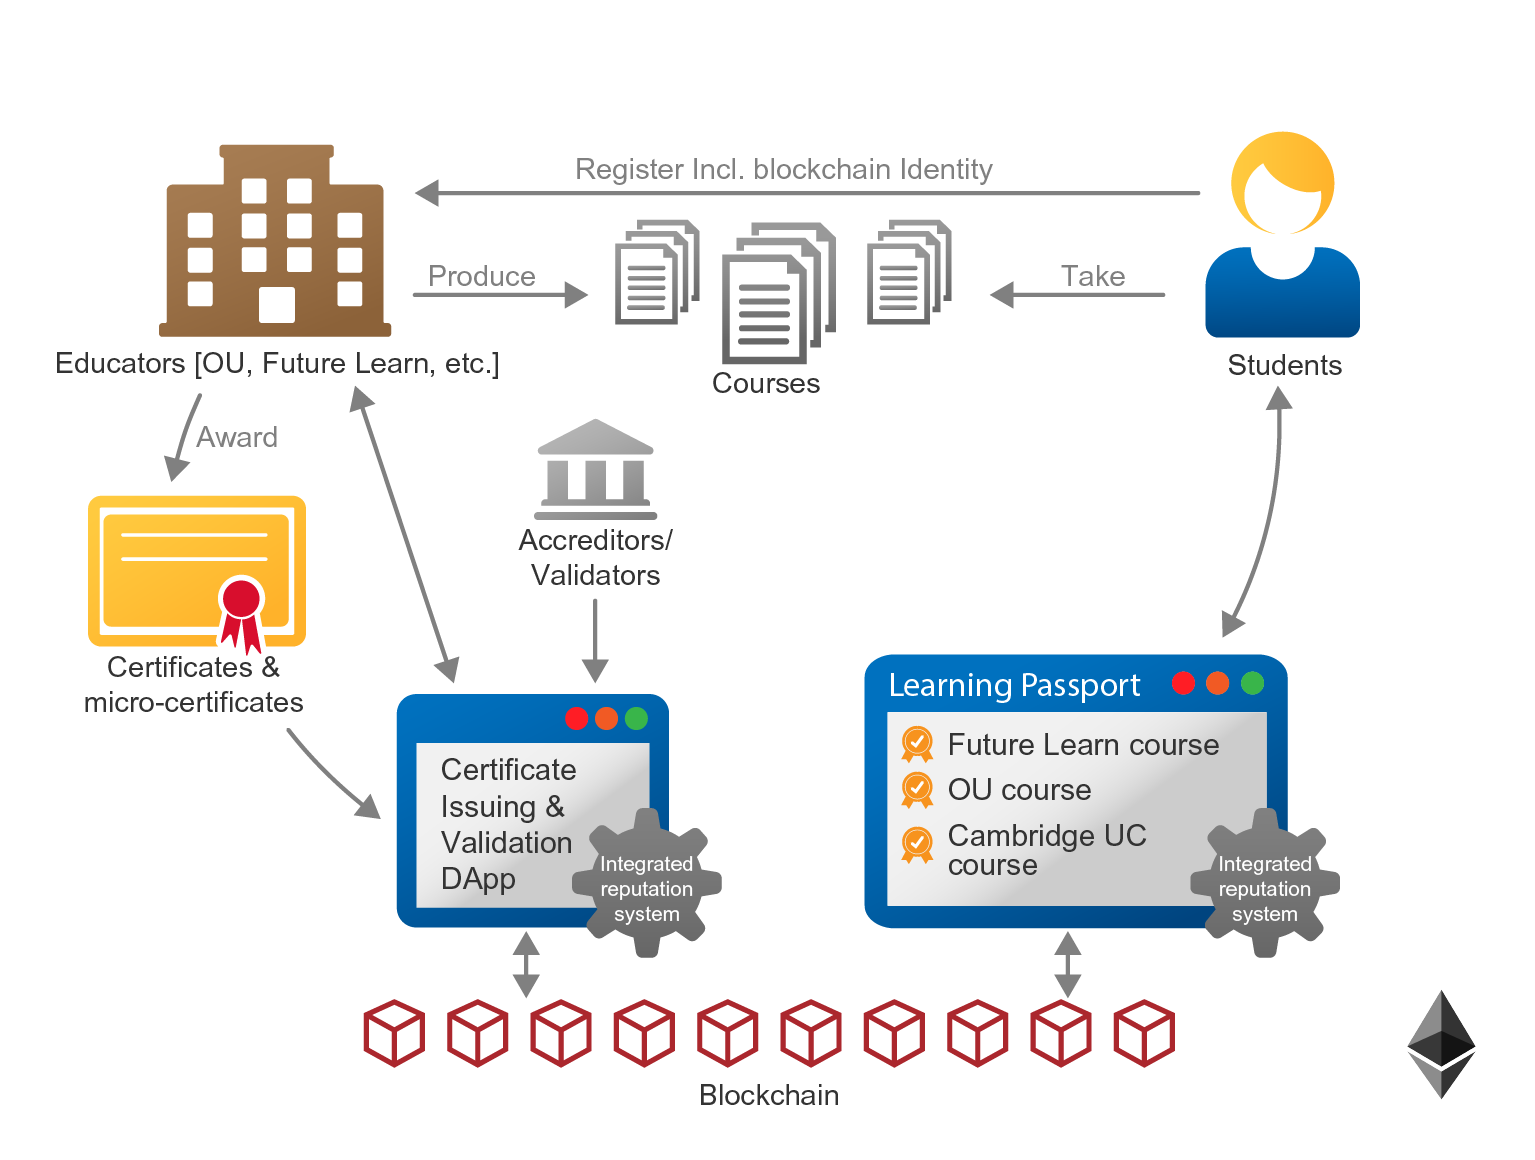
\includegraphics[width=.7\textwidth]{passport}
  \caption{A scenario of how blockchains and smart contracts can support accreditation and certification in higher education} 
  \label{fig:passport}
\end{figure} 

% A Learning Passport \DJ{}App would enable learners to easily view and manage all recognition of their learning no matter if informal or formal. These might include badges collected for course completion from MOOCs and formal degree course certificates. 
% Each of these two \DJ{}Apps would incorporate evaluation and reputation services. Certificates can be verified partly through reputation, but also be stored as credentials on the platform. For example, a verified credential proving certain prerequisites at one institution can allow a student to easily enroll in a higher level course at another. This allows the platform to operate with little overhead. Evaluation and reputation services would allow teachers and students to match their learning styles effectively. It will also set the stage for self-regulation of the system. Semantics can help in supporting interoperability issues in the above scenario. Namely:
% \begin{itemize}
%     \item Mapping from university and educational establishment data structures into the data structures as required by blockchain transactions and for the smart contracts.
%     \item Semantically, indexing template smart contracts and transactions for re-use.
%     \item Mapping between the Learning Passport data format into arbitrary certification and badging systems.
% \end{itemize}

\subsection{Credential Certification via Ethereum Virtual Machine}

Central mediation of services has become a bulwark of the Web. 
Common functions that are typically in the domain of central authorities include escrow/dispute resolution (e.g. eBay, AirBnB), identity management (e.g. Google+, Facebook). 
The \emph{Ethereum project} as created a blockchain with a built-in programming language. 
It is a platform that creates a virtual machine designed to be run by all participants in the peer-to-peer ``mining'' network. 
The purpose of which is to allow people to write decentralized applications (stylized as \textit{\DJ{}apps}) using blockchain technology. 
Although the project is relatively new \cite{wood2014ethereum} it holds the promise of affording users the ability to read and write to a blockchain both (quasi-Turing complete) executable code as well as data. 
The Enigma project from MIT is a related effort \cite{zyskind2015enigma}.

Traditional applications and web portals act mainly as a unified front-end to aggregate clients and provide the services of a particular entity. 
As conceptualized by the Ethereum project a \DJ{}app is a tool for people and organizations to act as counter-parties to an exchange without any such centralized intermediary.
A \DJ{}app is an application which serves some function for its users, but which has the salient characteristic that the application does not depend on the ongoing existence of any one actor. 
Some examples of proto-\DJ{}apps include BitTorrent for file sharing and of course Bitcoin for currency. 
The goal of the Ethereum project is to allow developers to generalize peer-to-peer network and blockchain technologies for a myriad of purposes.

The \emph{Ethereum Virtual Machine} (EVM) is the runtime environment for \DJ{}apps.  It is completely isolated (sandboxed) such that code running inside the EVM has no access to network, other processes, or the local filesystem.
Essentially the EVM is aiming to become a blockchain (viz. large decentralized computing network) with a multiplicity of nodes that collectively have the ability to maintain an internal database, execute code and communicate among one another.
In subsequent sections we explore how \DJ{}apps can facilitate a series of novel methods for the symbiotic development of blockchain technologies and the Semantic Web as applied to contemporary education methodologies. 

One of the defining characteristics of the $21^{st}$ century has been the proliferation of highly novel mediums by which people all over the world are empowered to share and consume information. 
This paradigm has given rise to new industries and is having a profound impact on well established ones. 
In this environment new opportunities are created for individuals with the appropriate proficiencies and accordingly the process of skill acquisition is one of the strongest indicators of societal change.

\subsection{Recognition of Credentials}

\emph{Massive Open Online Courses} (MOOCs) typically comprise a lecture series including accompanying material, focused on a particular subject, created for broad distribution across the Internet with largely unrestricted access for interested participants. 
Since their inception MOOCs have consistently attracted staggering numbers of students, typically in the hundreds of thousands.  
What is the reason for this popularity?

The increasing sophistication of statistical models that drive automation processes and machine learning are having a substantive impact on the economic landscape and are projected to make large numbers of jobs redundant in the coming years. 
This situation is merely one example in a cadre of changes that reflect a larger trend which might be described as something approaching a tectonic shift in the fundamental factors that drive the global economy. 
The rapid growth and demise of platforms and frameworks, the tools that support the dynamic response of industry to the increasingly mercurial needs of consumers, fuels a demand for educational resources that can keep abreast of the core competencies needed to distinguish oneself in the highly competitive job market.

\subsection{Impetus to Success}

The New York Times labeled 2012 ``the year of the MOOC'' \cite{laurapappano2012} with the emergence of a number of successful online education platforms backed by large industry actors and top universities.
In the intervening years there has been a diminution in the amount of media attention surrounding MOOCs, due (in no small part) to the low numbers of students that remain involved with the course through to successful completion. 
It has been strongly conjectured that one of the primary causes behind these disappointing statistics is the fact that there is considerable uncertainty as to how exactly the achievements benchmarked in MOOCs should be recognized. 
We focus particularly on MOOCs as an application scenario for using blockchain technology to certify learning achievements.
Learning today takes place in a context of new interactions between formal and informal learning. 
This is characterized by the changing role of teachers, the impact of social media and the students active participation in the design of learning activities.
Expertise in a domain might be gained through participation in a Meetup event, continued involvement in a question answering platform, thoughtful contemplation of recorded video content, or through a multiplicity of channels. 
All of these non-traditional educational mediums are marginalized by our current system of honouring credentials.

\subsection{Learning passport}

\autoref{fig:passport} shows a scenario of how a smart contract platform such as Ethereum could support micro and standard accreditation within a higher educational setting.
Educational establishments including universities and MOOC providers such as \emph{FutureLearn}\footnote{\url{http://www.futurelearn.com/}} develop and deploy courses and award recognition of student achievement through certificates, micro-certificates and badges. 

Students take courses and gain recognition after registering for and completing courses through certification. 
In an era of re-skilling and lifelong learning\footnote{No 21 year old on completion of a bachelor's degree will have gained all the skills he or she requires for the rest of his/her life} students will increasingly take a variety of courses from a variety of providers over a longer period of time. 
There is a need in this context for students to be able to collect and store all their informal and formal qualifications in a fashion that makes these easily accessible to relevant parties such as potential employers and educational organisations. 
The above process can be supported by two decentralized blockchain based applications (\DJ{}Apps) running on the Ethereum network. 
A \emph{Certificate Issuing and Validation} \DJ{}App would handle the publication of signed certificates within a blockchain. 
Secure signatures would tie all certificates to the specific issuing educational institution and the receiving student. 
Because of the nature of blockchains the certificates would remain valid even if the issuing organisation ceased to exist. 
Recently, the University of Nicosia has placed all the certificates for its free introductory MOOC ``\textit{An Introduction to Digital Currencies}'' within the Bitcoin blockchain\footnote{\url{http://digitalcurrency.unic.ac.cy/certificates}}.

A \emph{Learning Passport} \DJ{}App would enable learners to easily view and manage all recognition of their learning no matter if informal or formal. 
These might include badges collected for course completion from MOOCs and formal degree course certificates. 
Each of these two \DJ{}Apps would incorporate evaluation and reputation services. 
Certificates can be verified partly through reputation, but also be stored as credentials on the platform. 
For example, a verified credential proving certain prerequisites at one institution can allow a student to easily enroll in a higher level course at another. 
This allows the platform to operate with little overhead. 
Evaluation and reputation services would allow teachers and students to match their learning styles effectively. 
It will also set the stage for self-regulation of the system. 
Semantics can help in supporting interoperability issues in the above scenario, namely:
\begin{itemize}
    \item Mapping from university and educational establishment data structures into the data structures as required by blockchain transactions and for the smart contracts.
    \item Semantically, indexing template smart contracts and transactions for re-use.
    \item Mapping between the Learning Passport data format into arbitrary certification and badging systems.
\end{itemize}

\section{Decentralized Application (\DJ{}App) for Education}

As stated above Ethereum is a platform intended to facilitate the development of decentralized applications (\DJ{}apps) using blockchain technology. 
A foundational ingredient in the efficient operation of programs on this distributed application platform is ``Ether''. 
This is a form of payment made by the users of the network to the machines executing their code. 
Ether is the incentive ensuring that developers write applications that do not waste resources, e.g. running endless loops on the platform, it also ensures that users are compensated for the contribution of their computation time and/or memory space.

Recent work at The Knowledge Media Institute (KMi), research and development arm of The Open University, has been centered around the implementation of a decentralized application, which enables crowd-based recognition of educational activity on the \emph{FutureLearn} and \emph{OpenLearn}\footnote{\url{http://www.open.edu/openlearn/}} platforms. 

\begin{figure}[!ht]
  \centering
      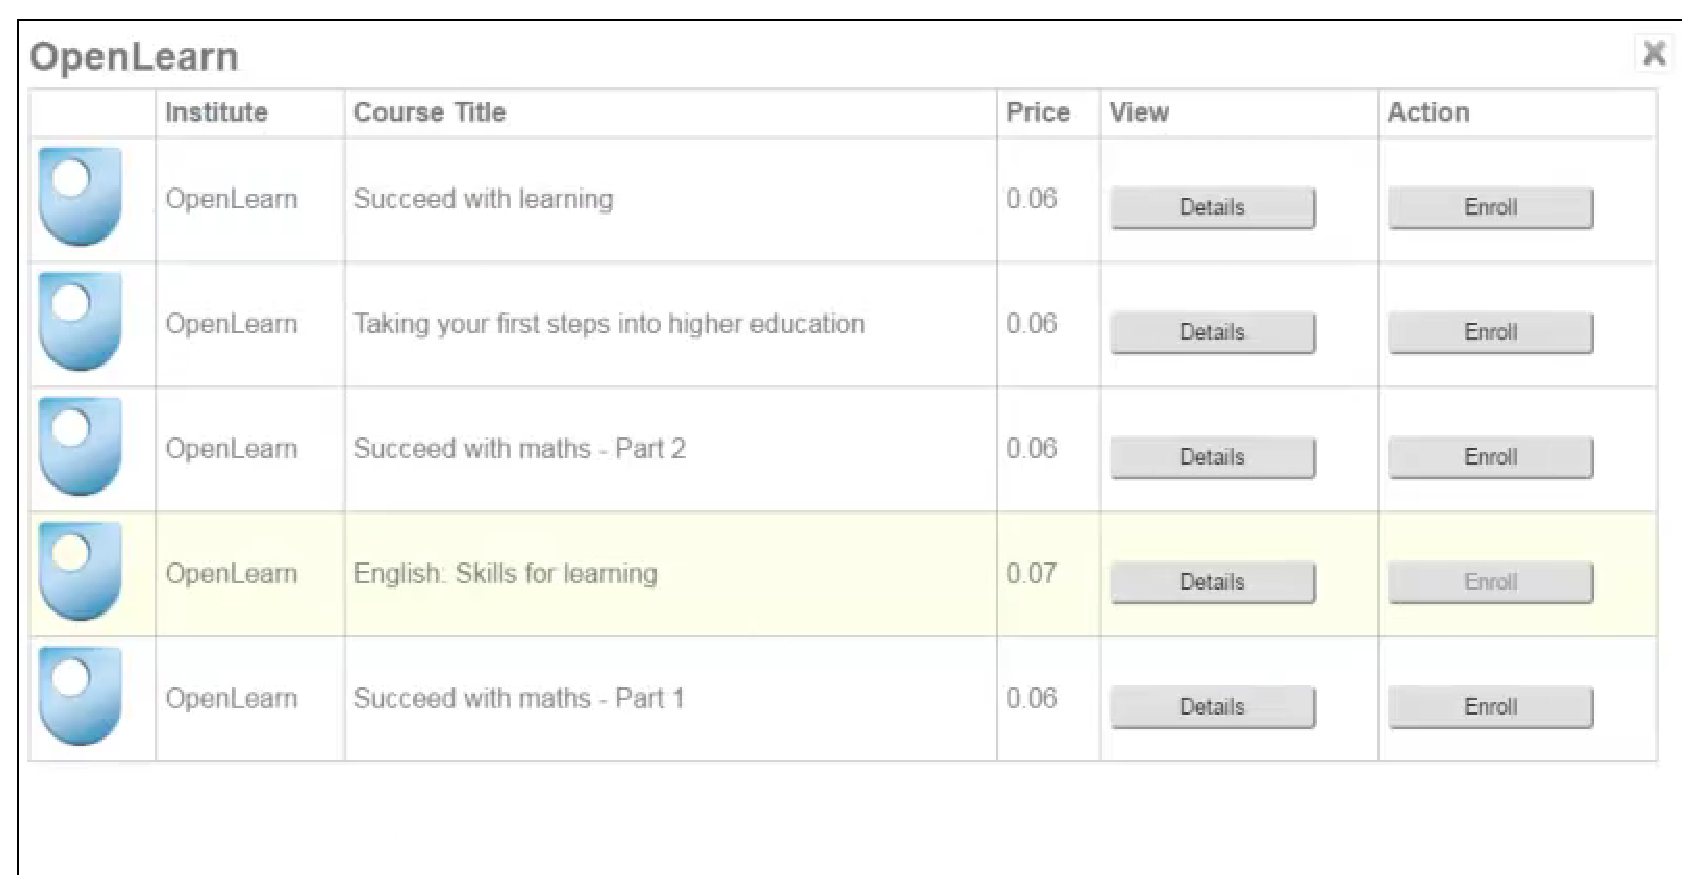
\includegraphics[width=0.69\columnwidth]{plat}
  \caption{Platform view.}
    \label{fig:xyz}
\end{figure}

The \DJ{}apps provides students the ability to enroll in courses using Ether funds, receive certifications of achievement, called ``awards'' and aggregate the awards in a sharable common interface. 
In this ecosystem the users, viz. students and administrators, manage enrollment, and remuneration (using Ether), in addition to the assignment of credentials all on the blockchain.   
On the Ethereum network a \DJ{}app consists of two parts: a frontend, written in HTML, and a backend, essentially the database of the application. 
We have developed a fully functional prototype of such a system, demonstrated in \autoref{fig:xyz}. 

\begin{figure}[!ht]
  \centering
      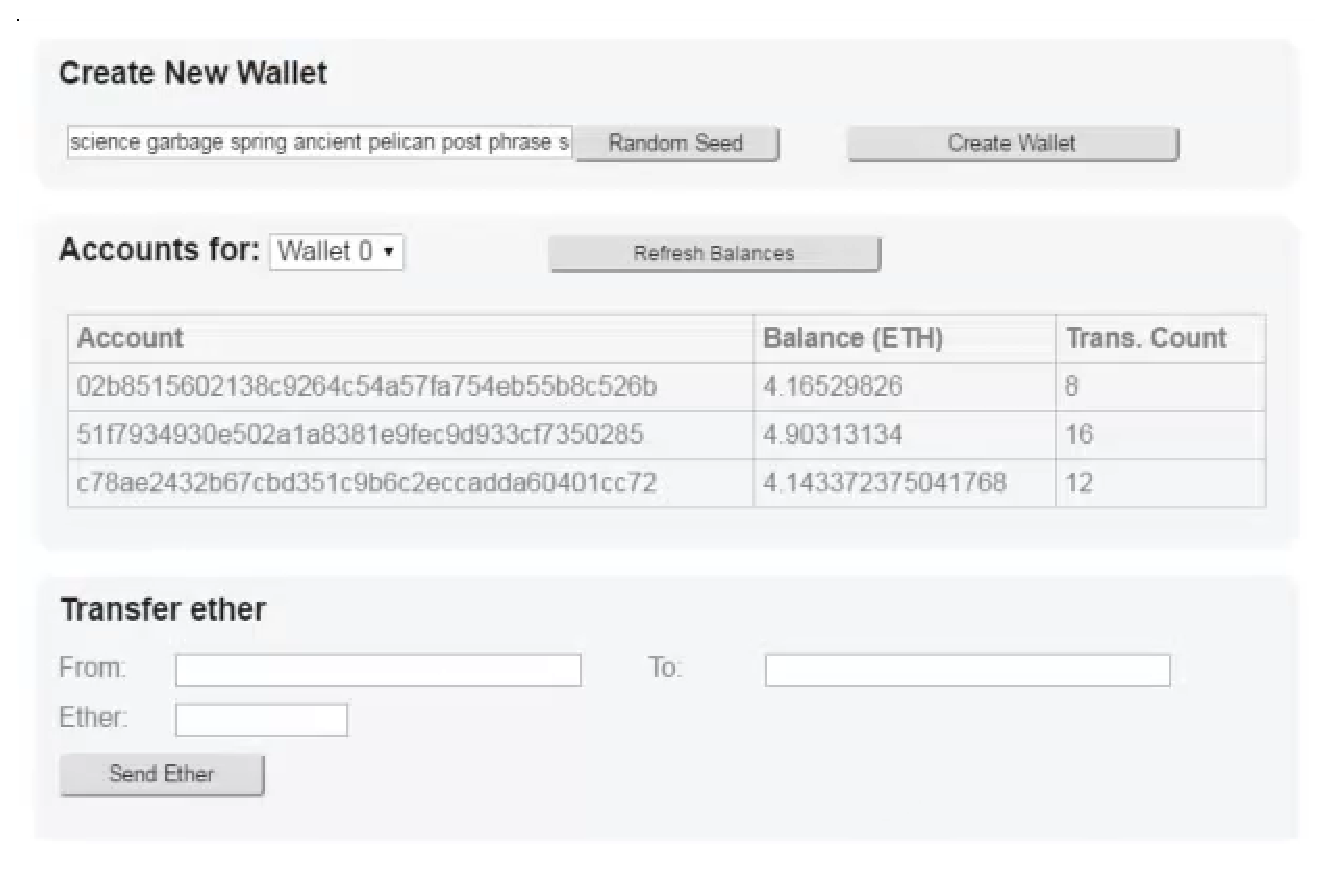
\includegraphics[width=0.69\columnwidth]{wallet000}
  \caption{Prototype of ``\textit{Student Browser}'' frontend.}
\end{figure}

From the main element ``My Wallets'' view students manage their Ether (available funds) account. 
Users create one or more wallets, and use them to transfer funds between different actors, e.g. a transmission of their Ether to an online learning platform such as \emph{FutureLearn}. 
There is a profile area wherein users can establish their identity by associating it with a known public key.
Accordingly an individual wallet account is bound to a name and an icon. 
Subsequently this account can be indicated as the ``current account'' and used to enroll in a course. 

\begin{figure}[!ht]
  \centering
      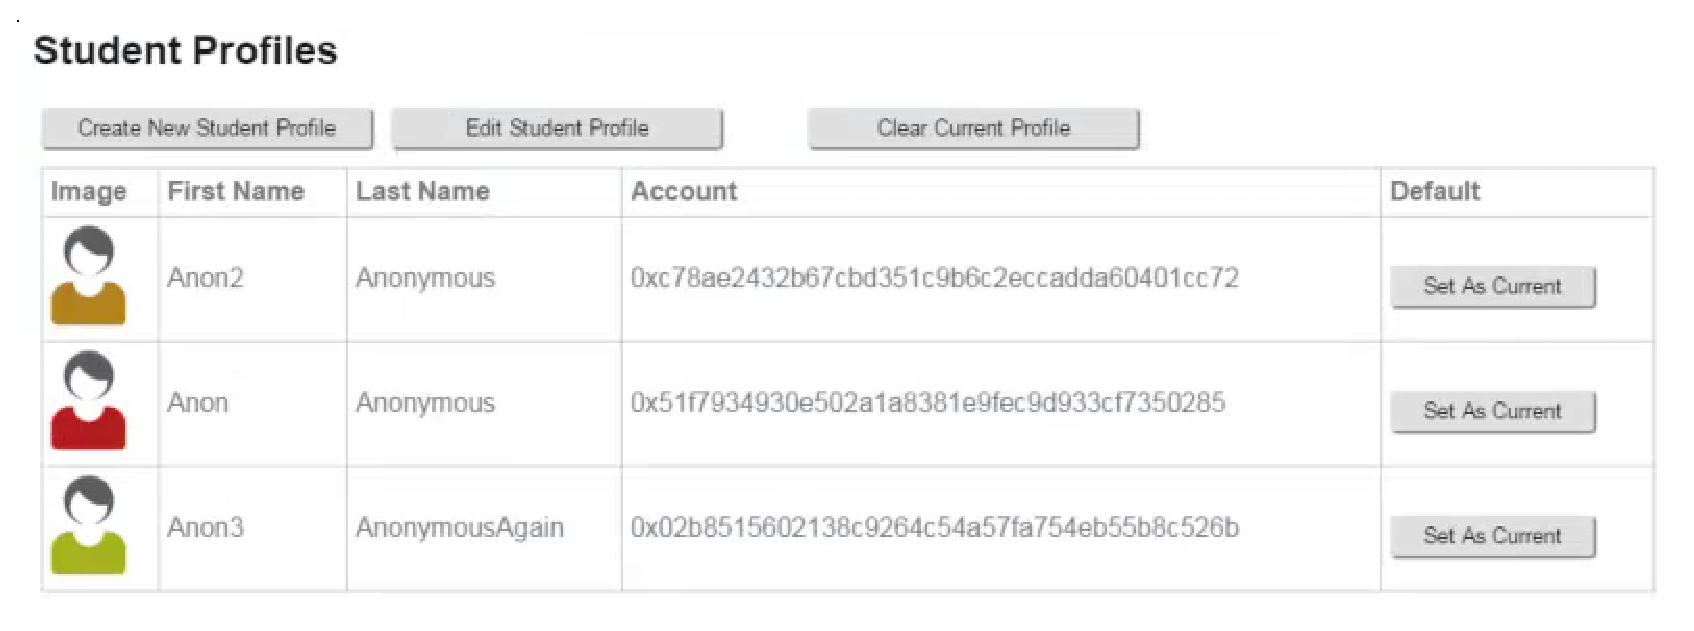
\includegraphics[width=0.69\columnwidth]{stupo}
  \caption{Dashboard view of multiple different user accounts.}
\end{figure}

The embedded \DJ{}app Store contains course selections from multiple sources, among them both \emph{FutureLearn} and \emph{OpenLearn} and are anticipating content from \emph{Fraunhofer Academy}\footnote{\url{http://www.academy.fraunhofer.de/en.html}} and \emph{SlideWiki}.

To register for a course in the system a user must initiate the process with a click-through of the ``Register'' button, this will prompt a pop-up box with a password input screen, since subsequently a monetary transaction (using Ether) will take place. 

\begin{figure}[!ht]
  \centering
      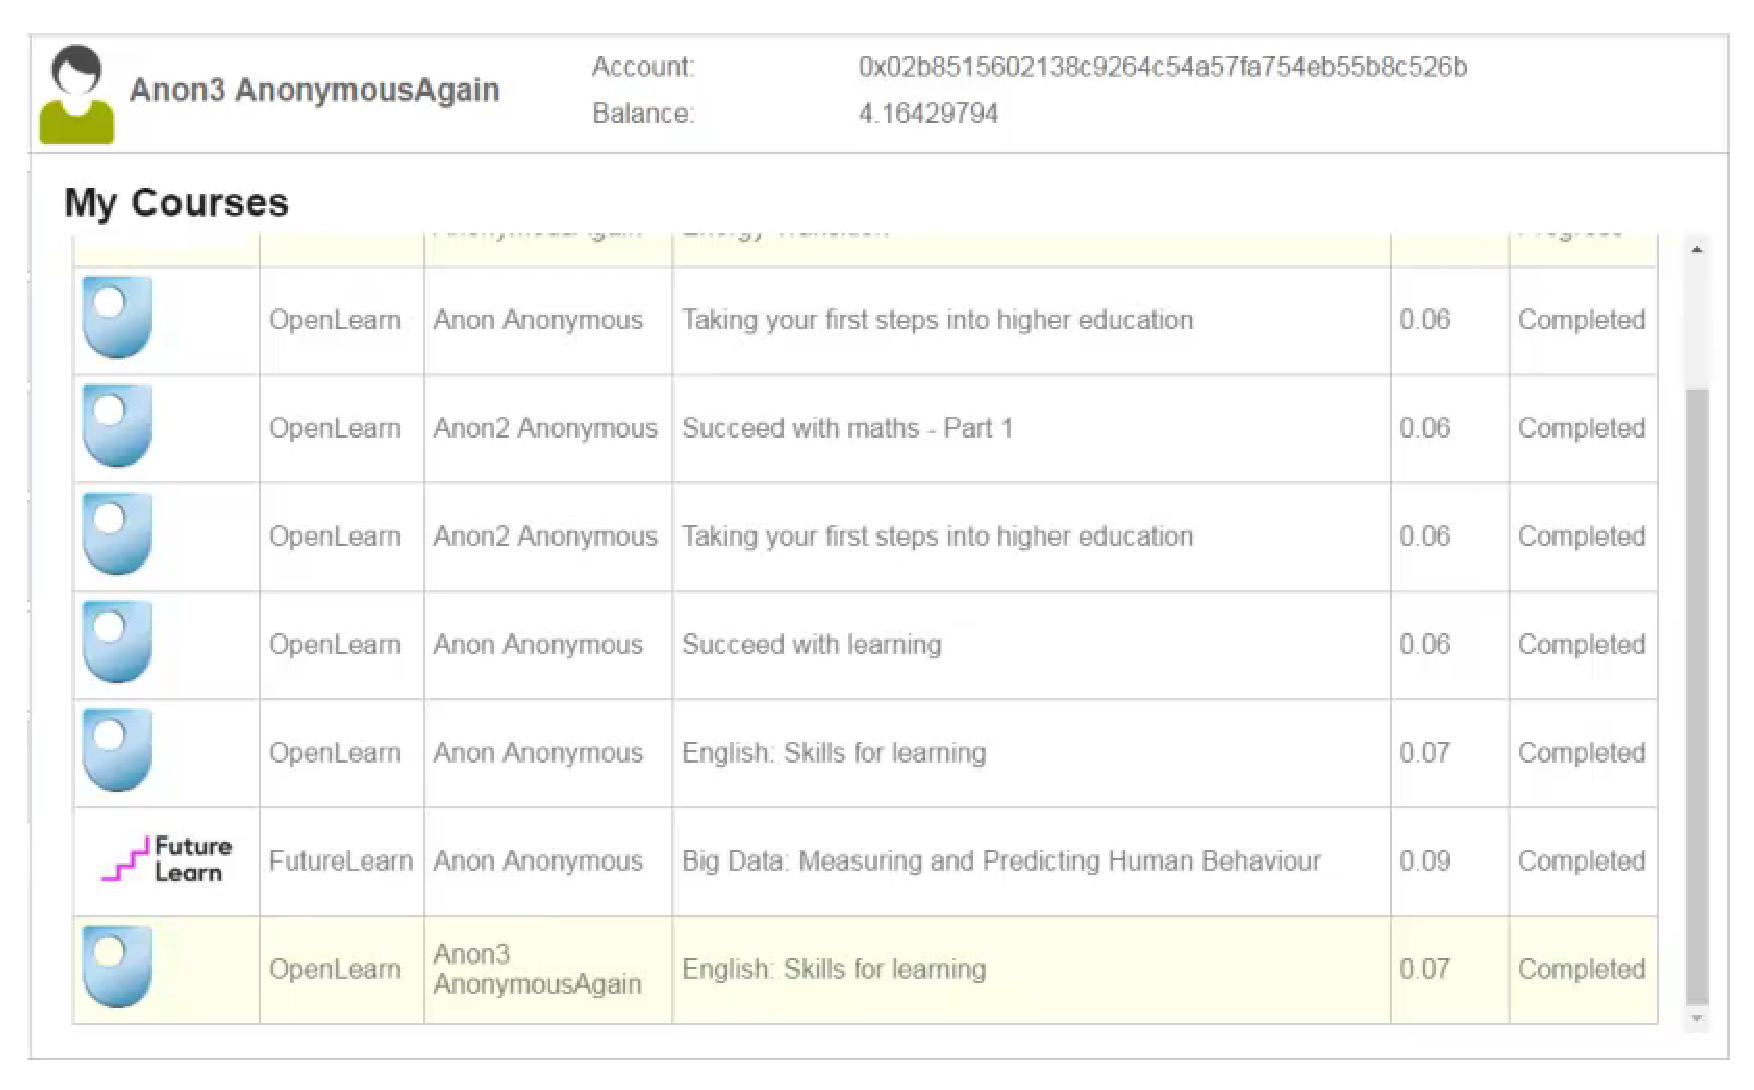
\includegraphics[width=0.69\columnwidth]{kor}
  \caption{Course Dashboard.}
\end{figure}

Concurrently with this interchange we can see a transaction which is generated on the blockchain, it will remain pending until it is mined, this is viewable in a partition of the browser window depicted in \autoref{fig:abc}. 

\begin{figure}[!ht]
  \centering
      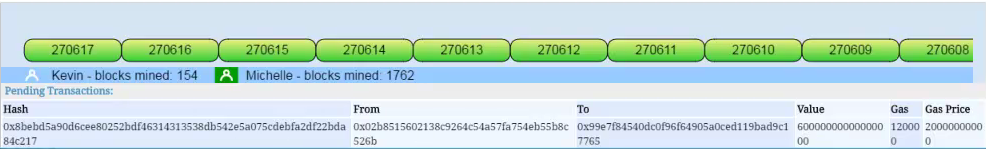
\includegraphics[width=0.69\columnwidth]{blockchain_dapp}
  \caption{Blockchain transaction.}
        \label{fig:abc}
\end{figure}

Mined (confirmed) blocks are represented by the numbered green ovals, unconfirmed blocks will appear as red. 
There is a transaction hash, and the two hashes representing sender (From) and receiver (To). 
Once the block has been successfully mined it will be added to the list of courses pending. One additional exchange (separate from the transactions that pay for enrollment in the course) facilitates its delivery to the course dashboard of the user.
On the current environment this process is instantaneous, on a larger network, e.g. the web-scale Bitcoin blockchain, as currently implemented, to confirm with certainty might take the amount of time required to process a new block, i.e. not more than 10 minutes. Once the course has been completed the administrator can log-on to issue the award. 
After the block containing the award has been mined it can be found in the ``Awards List'' of the associated student. 
% The following code snippet represents a component of an Ethereum ``smart contract'' for an educational institute to offer courses. 
Note that no students are using this course demo for enrolment as it is currently merely a proof of concept.

\begin{figure}[!ht]
  \centering
      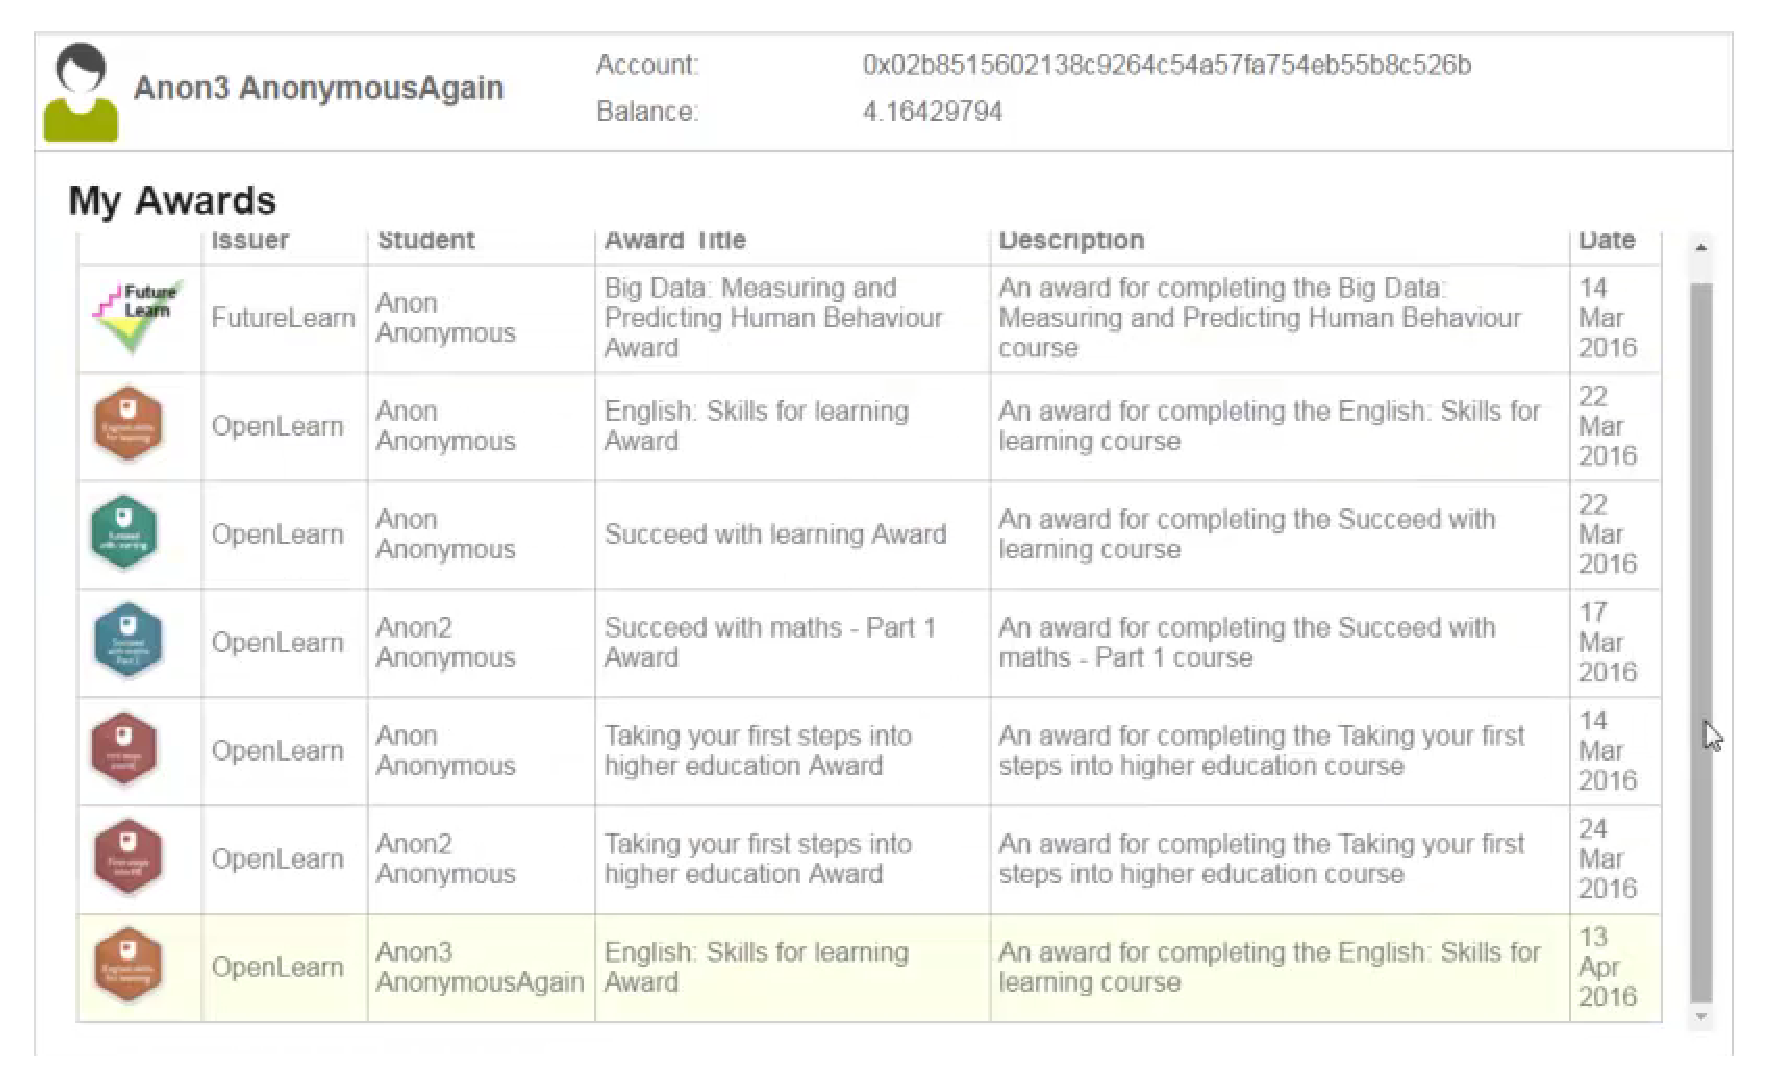
\includegraphics[width=0.69\columnwidth]{awardz}
  \caption{Awards view.}
\end{figure}
\begin{figure}[!ht]
  \centering
\begin{lstlisting}
	function getCourses() public returns
	(address[] availablecourses){
		availablecourses = courses;
		return availablecourses;
	}
	
	function addCourse(address course) 
	public onlyOwner returns (bool success){
		bool exists = false;
		success = false;
		uint i=0;
		uint count = courses.length;
		address next;
		for (i=0; i<count;i++) {
			next = courses[i];
			if (next == course) {
				exists = true;
			}
		}
		if (exists == false) {
			success = true;
			courses.push(course);
		}
	}
\end{lstlisting}
  \caption{Ethereum ``smart contract'' snippet}
\end{figure}
% % \section{Related Work} 

\subsection{Open Badges}

The work we have carried out thus far in the domain of the Semantic Blockchain is largely a continuation of the achievements recorded by the initiatives described in this section. 
The Mozilla Foundation and Peer2Peer University, in collaboration with The MacArthur Foundation, contributed significantly to the field of credential assignment in the context of non-traditional education through the publication of a well known white paper on the subject of modular accreditation~\cite{schmidt2011can}. 
The initiative is known under the name ``Open Badges for Lifelong Learning''.  
The purpose of which is to support skill development and lifelong learning for ``real results'', e.g. job placement and advancement ~\cite{themozillafoundationpeer2peeruniversityincollaborationwiththemacarthurfoundation2011}.

The essence of a digital open badge is a standardized way to conveniently demonstrate that one has achieved a given degree of competency in a particular domain. 
Through close cooperation with credible organizations Open Badges facilitates the process of skill, interest and achievement verification. 
The system is based on an open standard, such that one is free to combine multiple badges from different issuers in a comprehensive accomplishment narrative. 
The aim of this platform is not restricted to the Web and should transcend the digital medium to be applicable to work performed online as well as offline.
Through the shared technical standard Open Badges facilitates a process of garnering recognition for the things one learns as well as the things one is able to teach. 
Anyone who satisfies the standard can award badges. 
There is a vibrant community of contributors and partners supporting this effort, such as NASA, the Smithsonian, Intel, and the American Girl Scouts. 
Originally the badges infrastructure envisioned a decentralized server structure, but the incentives for providers to run these servers were never strong enough to maintain such an environment.
For this reason it appears that the blockchain is a better foundation, as it is run by self-interested entities but can openly be utilized for broad community-based initiatives ~\cite{philippschmidt2015}.

\subsection{Blockchain Certificate Issuance}

We have alluded to the fact that a blockchain database is durable, time-stamped, transparent, and decentralized. 
These characteristics are useful attributes in the management of a reputation system. 
We can consider reputation as a type of currency that enables access to social capital, as opposed to financial capital.
The MIT Media Lab is currently issuing blockchain certificates in accordance with the following procedure:

\begin{enumerate}
\item Create a digital file that contains basic information such as:
\begin{enumerate}
    \item the name of the recipient
    \item the name of the issuer
    \item an issue date
\end{enumerate}
\item Subsequently the contents of the certificates are signed using a private key to which only the Media Lab has access 
\begin{enumerate}
    \item append that signature to the certificate itself
\end{enumerate}
\item Next create a hash, which is a short string that can be used to verify that nobody has tampered with the content of the certificate. 
\item Finally use the private key once again to create a record on the Bitcoin blockchain which states that a certain certificate was issued to a certain person on a certain date
\end{enumerate}

This system makes it possible to verify who a certificate was issued to, by whom, and validate the content of the certificate itself. 
Currently it uses the Bitcoin blockchain by way of the OP\_RETURN field. 
OP\_RETURN is a script operation code used to mark a transaction output as invalid. 
Since the data after OP\_RETURN are irrelevant to Bitcoin payments, arbitrary data can be added into the output after an OP\_RETURN. 
The hash value of the MIT Media Lab is stored in this OP\_RETURN segment.
The current version creates a separate transaction for each certificate.
Future versions of the software could store all hashes in one Merkle tree and only the Merkle root might be stored in the OP\_RETURN, referring back into the blockchain approximately once every day. 

\subsection{Industry Interest}

Sony Global Education, Inc. a division of the multinational conglomerate company Sony Corporation is the foremost industry actor to announce an interest in the adaptation of blockchain technology to the field of education \cite{sonyglobaleducation2016}.
They are pioneering an effort to realize a solution to enable open and secure sharing of academic proficiency and progress records by leveraging the security properties inherent in the blockchain to facilitate the encrypted transmission of data, such as an individual's academic proficiency records and measures of progress, between two specified parties.
Regarding the initiative Sony Global Education has released a public statement to the effect that,

\begin{displayquote}
``\textit{The technology has the potential to realize an entirely new infrastructure system for sharing records securely over the network in any number of ways, opening new doors of possibility for academic records and how they are assessed. For example, after taking an examination to demonstrate his or her academic proficiency level, an individual could direct the testing organization to share the test results with one or more third-party evaluating organizations. This would be a first if implemented on a system-wide basis}''
\end{displayquote}

while notably vague as to the details of the implementation, from this statement we can clearly discern the strong motivation for a solution that under-girds such efforts. 
It enables network users to freely and securely transfer permissions, without the need for an established relationship of trust between network participants, and in such a way that damaging or tampering with programs and data is prohibitively difficult.


\section{Overview}

This chapter represents a first statement on the relationship between blockchains and the Semantic Web, and accordingly we sought to encompass a comprehensive overview that includes all pertinent activity we have thus far undertaken in the space such that it might serve as a catalyst for further development.
We strongly feel that many lessons on how semantics has been aligned with the Web infrastructure could be applied to blockchains. 
The proposed application scenario of MOOCs was selected not for the extraordinary utility that this paradigm provides but to illustrate the concept that the ability to trace an exchange or transaction through the blockchain can provide a social benefit, alleviating the need for holders of credentials to verify their accomplishments ad infinitum, a common problem for those who have obtained degrees abroad.  
Moreover, it seems clear that online learning and the need for new methods to fill existing skills gaps will continue to develop going forward.




